%% This is an example first chapter.  You should put chapter/appendix that you
%% write into a separate file, and add a line \include{yourfilename} to
%% main.tex, where `yourfilename.tex' is the name of the chapter/appendix file.
%% You can process specific files by typing their names in at the 
%% \files=
%% prompt when you run the file main.tex through LaTeX.
\chapter{Transforming For Improved Fit}
The previous chapter showed that the quality of the solution generated by KBRL
can be improved by transforming the state space of the MDP.
The chapter also showed that constructing a transform that makes the value
function easier to represent requires one to already know the value function.

We now describe an algorithm that attempts to solve this chicken-and-egg
problem iteratively. Section 1 proposes a novel curve-fitting framework,
Fit-Improving Iterative Representation Adjustment (FIIRA),
which takes a regression scheme and a transform generator, and produces a
more powerful regression scheme.
Section 2 describes a specific transform generator for use in FIIRA.
Section 3 discusses the results of combining that transformer with a kernel
smoother.
Section 4 describes an FIIRA approach to KBRL.
Finally, Section 5 provides some implementation considerations.

\section{Fit-Improving Iterative Representation Adjustment}
The problem statement of curve-fitting is as follows: given a set of training
points, $D = \{(x_i,y_i)\ |\ i = 1, \ldots, n\}$, of point-value pairs with
$y_i = f(x_i)$ for some function $f : X \to \mathbb{R}$,
produce a function $\tilde f$ to approximate $f$ well, for some measure of
approximation quality.

A regressor, $r$, is a procedure for producing fits from some space of
functions, $\mathcal{F}_r$.
If $f$ is not well approximated by any function in $\mathcal{F}_r$,
this fit is guaranteed to be poor.
One way to fix to this problem is to transform the domain of $f$ and work in a
space where $f$ \textit{is} well approximated. Choosing such a transform
requires prior knowledge or assumptions about $f$.

What can one do if no information about $f$ is available?
Ideally, one would infer a transform directly from the data.
An interesting way to go about doing this would be to pass $D$ to the
regressor,
then use the approximation produced to guess a transform $\Phi$ such that
$f_\Phi$ is in or near $\mathcal{F}_r$.
Algorithm 1 describes a framework for doing this.
The procedure takes as input a dataset, $D$; a regressor, $REGR$;
and a transform generator, $TF$.

\begin{algorithm}
\caption{Iterative Representation Adjustment for Improved Fit}\label{FIIRA}
\begin{algorithmic}[1]
\Procedure{FIIRA}{$D,\ REGR,\ TF$}
	\State $\Phi_0 \gets x \mapsto x$
          \Comment{The identity transform}
	\State $i \gets 0$
        \State $D_0 \gets D$
	\Repeat
		\State $\tilde f_{i+1} \gets REGR(D_i)$
		\State $\Phi_{i+1}\gets TF(\tilde f_{i+1}, D_i)$
		\State $i \gets i+1$
                \State $D_i \gets \{(\Phi_{i+1}(x), y)\ |\ (x,y) \in D_{i-1}\}$
	\Until{$\tilde f_{i+1} \approx \tilde f_i}$
           \Comment{Or until some measure of error minimized}
	\State \textbf{return} $x \mapsto f_{i+1}(\Phi_{i+1}(x))$
\EndProcedure
\end{algorithmic}
\end{algorithm}

It may not be immediately clear what leverage this technique has to offer.
To see what it can do, consider the case where the regressor
creates polynomial fits of order $p$ and the transform generator
creates polynomial transforms of order $q$.
Applying $k$ iterations of FIIRA will yield a polynomial fit of order
$p + kq$.

I was unable to find anything like FIIRA in the function approximation
literature so I cannot cite any relevant theorems or results.
A formal analysis of the properties of FIIRA
is outside the scope of this thesis and is left for future work.
What follows is an empirical study of FIIRA for the special
case where the regressor is a local-averaging kernel smoother
and the transform generator is the Wrinkle-Ironing Transformer
described below.

\section{Dimension-Adding WIT}
The regressor used in KBRL is a local-averaging kernel smoother.
An FIIRA approach to KBRL requires a transformer that makes functions
easier to represent by kernel smoothing.
If we accept wrinkliness as a measure of representation difficulty,
it follows that the desired transformer is one that produces
Wrinkle-Ironing Transforms.
WITs stretch out the parts of the space where a function is steep
and squash the parts where it is flat.
I now describe a WIT that does this by adding a dimension to the domain.

Consider a transformer which, given a function $f$ with domain $X$, 
maps every $x \in X$ to $x | f(x)$ (the bar represents concatenation).
The transform generated stretches $X$ into $d+1$ dimensions in a way that
pulls apart points that differ in value.
Figure 4-1 demonstrates how this works.

\begin{figure}[!htb]
  \minipage{0.5\textwidth}
    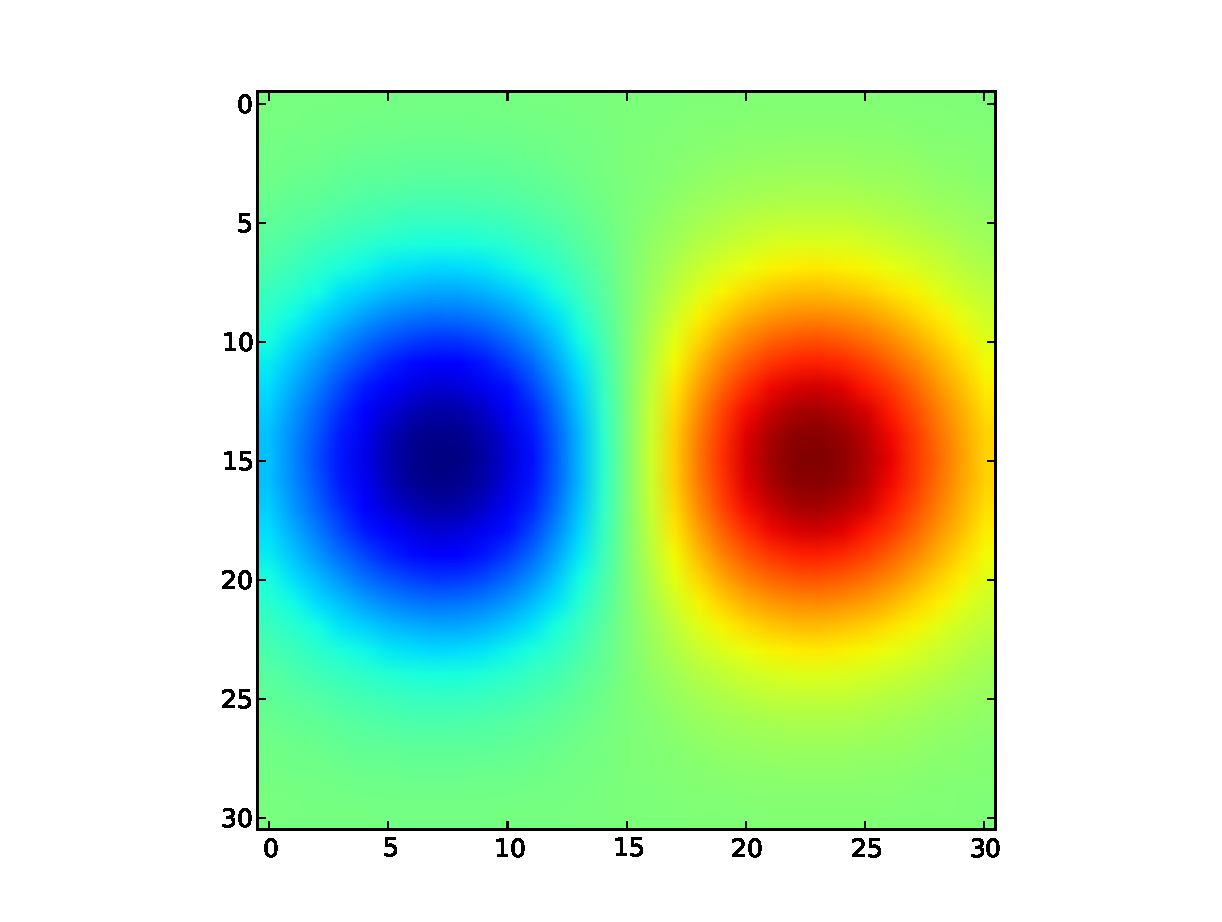
\includegraphics[width=\linewidth]{figs/bumps.pdf}
  \endminipage\hfill
  \minipage{0.5\textwidth}
    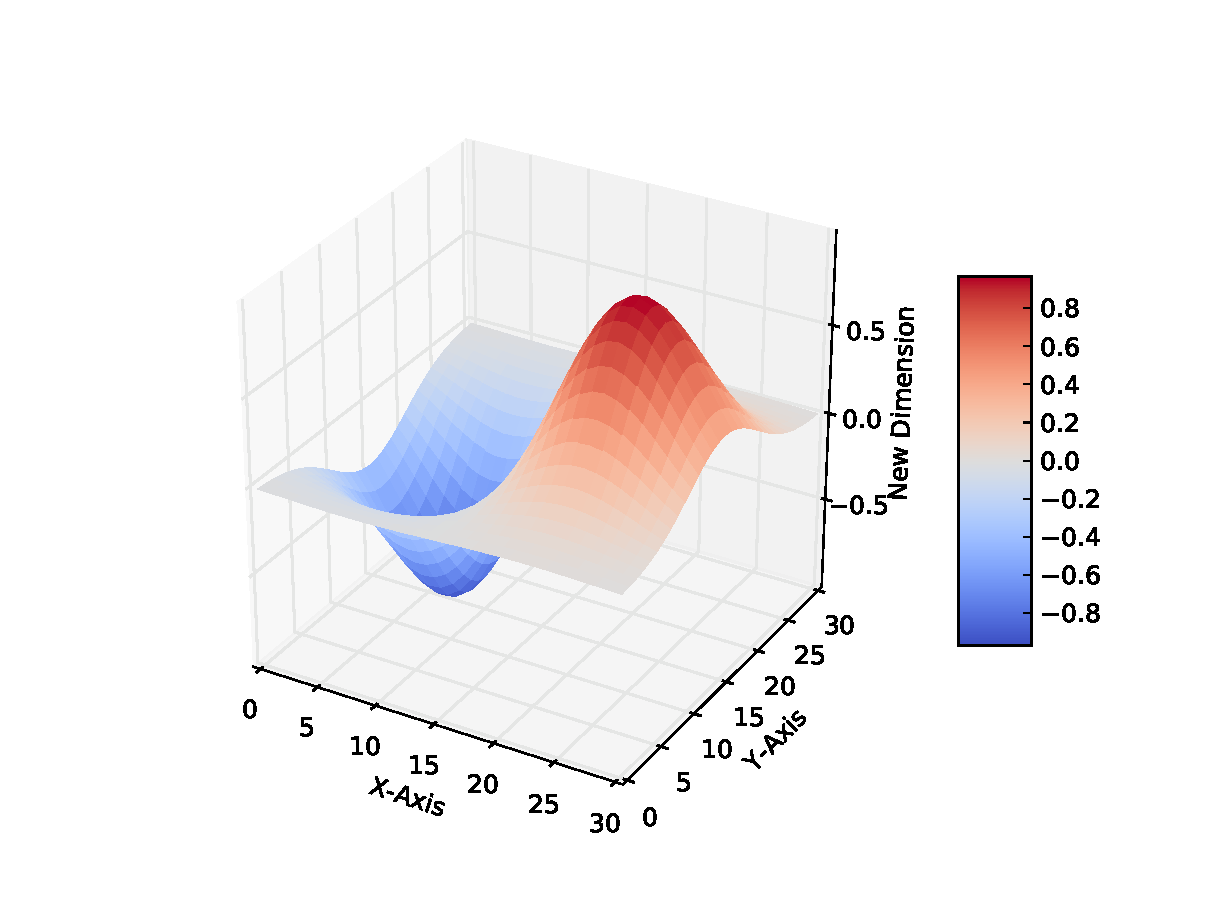
\includegraphics[width=\linewidth]{figs/tfbumps.pdf}
  \endminipage
\caption[Dimension-Adding WIT example]
{The figure on the left is a heatmap of some function.
The areas in red are where it attains a high value and the ones in blue
are where it attains a low value.
The figure on the right shows the transformed domain of the function.
The red areas are pulled up and out of the page while the blue ones are pushed
down and into the page. The areas where the domain is stretched most are
where the function has the steepest slope.}
\end{figure}

This transform does what we want, but it has two problems.
The first problem is that it is sensitive to the scale of $f$.
The fix is to normalize $f$ by its inverse target slope $\mu_f$; this way
$f$ has the same spread as its domain.
If we want to control the extent of the stretching, we can do so by also
scaling $f$ by a constant $\alpha$.
The second problem is that it is potentially diameter-increasing.
To counteract this, we should also normalize the new domain by 
a diameter-preserving constant, $c_0$.

With these changes, the $d$-dimensional vector, $x = (x_1, \ldots, x_d)$
gets mapped to $x' = c_0(x_1, \ldots, x_d, \alpha\mu_f\cdot f(x))$
The diameter-preserving $c_0$ is the ratio of the diameter of $X$ to the
diameter of the new space;
it satisfies  $\frac{1}{\sqrt{1+\alpha^2}} \leq c_0 \leq 1$.
Calculating $c_0$ exactly is difficult, so we just assume the lower
bound.
Note that this can potentially decrease the diameter, increasing the effective
bandwidth.

\begin{algorithm}
\caption{Dimension-Adding WIT}\label{dawitalg}
\begin{algorithmic}[1]
\Procedure{DAWIT}{$\tilde f$}
	\State $c_0 \gets \frac{1}{\sqrt{1+\alpha^2}}$
	\State\textbf{return}
          $x\mapsto c_0(x | (\alpha\mu_f\cdot\tilde f(x)))$
\EndProcedure
\end{algorithmic}
\end{algorithm}

To get a feel for what this transformer does, let us apply it to a concrete
example.
Assume the initial domain, $X$, is the unit interval $[0,1]$ and $f$ is a
function with range $[0,1]$ (so $\mu_f = 1$).
Calling \textit{DAWIT} on $f$ with $\alpha = 1.0$ will produce the
transform $x \mapsto \frac{1}{\sqrt{2}}(x, f(x))$.
This maps the unit interval to a curve in two dimensions.
Note that the maximum possible distance between points on this curve is $1$,
so the transform has not increased the diameter.
If we define a new function of two variables $f_2(x,y) = f(x)$ and call
 \textit{DAWIT} on it,
$X$ will be transformed into a curve in 3 dimensions; its points would take
the form $(\frac{x}{2}, \frac{f(x)}{2}, \frac{f(x)}{\sqrt{2}})$.
This curve can be rotated back into two dimensions to get the transform
$x \mapsto (\frac{x}{2}, \frac{\sqrt{3}}{2}f(x))$.
Calling \textit{DAWIT} in a loop $k$ times like this will transform the
domain to a $k+1$ dimensional curve which can be rotated to
$x \mapsto (\frac{x}{\sqrt{2^k}}, \sqrt{1-\frac{1}{2^k}}f(x))$.
Note how the domain is converging to a line---and not just any line.
It is converging to the best possible transform identified in the previous
chapter.
Since on every iteration, $x$ gets divided by $\sqrt{2}$,
this convergence happens exponentially quickly.
This happens for any connected $X$ and continuous $f$.

Now, let us see what happens when we run FIIRA with this transformer and
a kernel smoother.

\section{FIIRA with \textit{DAWIT} and a kernel smoother}
This section provides a discussion of the properties of the fit
generated when performing FIIRA with \textit{DAWIT} as the transformer and
a kernel smoother as the regressor.
For compactness, FIIRA with \textit{DAWIT} and a kernel smoother is referred
to as FDK.

\begin{claim} In the limit of infinite data and a bandwidth that shrinks at an
admissible\footnote{With admissibility as defined by Ormoneit et. al.
\cite{kbrl}} rate,
performing FDK to convergence produces the Platonic transform of the domain.
\end{claim}
\begin{proof} (sketch) If the bandwidth is sufficiently small,
$\tilde f_i \approx f$ for all $i$ because the approximation will be unaffected
by the representation.
Therefore the process would be like calling \textit{DAWIT} with the same
function on every iteration, which, as we saw above, results in convergence
to the Platonic transform.
This result implies that FDK preserves the statistical consistence
guarantees of kernel smoothing.
\end{proof}

\begin{claim} For any choice of bandwidth, dataset, and $\alpha$, performing
FDK will converge.
\end{claim}

\begin{proof} (sketch) To see this, let us first characterize the fixed points of
\textit{DAWIT}. A fixed point is a function whose domain does not get
distorted by the transform.
Let $f$ be a function that gets passed to \textit{DAWIT} and let
$a$ and $b$ be points in its domain.
 After the transform, the distance between $a$ and $b$ becomes
 $$\|\Phi(a)- \Phi(b)\| = \frac{1}{\sqrt{1 + \alpha^2}}
\sqrt{\|a-b\|^2 + \alpha^2\mu_f^2\cdot(f(a) - f(b))^2}.$$

This equals $\|a-b\|$ if only if $\mu_f \cdot |f(a) - f(b)| = \|a-b\|$.
For this to hold for all $(a,b)$ pairs, $f$ must have the same
slope everywhere.
Note that this is only possible if the domain of $f$ is one dimensional.
It follows that the fixed points of FDK
are datasets $D$ which produce $\tilde f$ such that
$\frac{\|x - x'\|}{|\tilde f(x) - \tilde f(x')|} = \mu_{\tilde f}$
for all distinct pairs of points $(x, x')$ in the domain of $\tilde f$ such
that $x \neq x'$.

The fixed points are not unique;
there are multiple datasets $D$ that result in such a $\tilde f$. An
elementary one is a set with only two distinct elements in the domain
(see proof in Appendix A).
A more interesting one is a set where all the $x_i$ are co-linear,
sorted by value, and spaced apart in such a way that $\tilde f$
is a line on its domain.
The first example is a stable fixed point and the second is an unstable one.
If the bandwidth is small enough, there can be stable fixed points
with more than two distinct elements.
For instance, if the mother kernel has compact support and a bandwidth less
than $\frac{\mathrm{diam}(X)}{c}$ for some $c$, then there exists a stable
fixed points with $c$ atoms (see proof in Appendix A).

On the $j^{th}$ iteration of FDK, points in $D_{j-1}$ are moved closer
together if the slope of $\tilde f_j$ between them is lower than
$\mu_{\tilde f_j}$.
Points that get moved closer together are likely to have similar values
on the next iteration, meaning they will get brought even closer.
This suggests that the domain is collapsing to a finite number of atoms.
\end{proof}

The fact that the domain collapses to a finite number of atoms implies
that FDK will produce a piecewise flat approximation to $f$.
Points that get mapped to the same atom will have the same value in the
limiting fit $\tilde f_\infty$.
Since there are a finite number of atoms $\tilde f_\infty$ will only take
a finite number of values. 
For a concrete example of how this happens, see Figures 4-2, 4-3, and 4-4.

\begin{figure}[!!!ht]
  \centering
    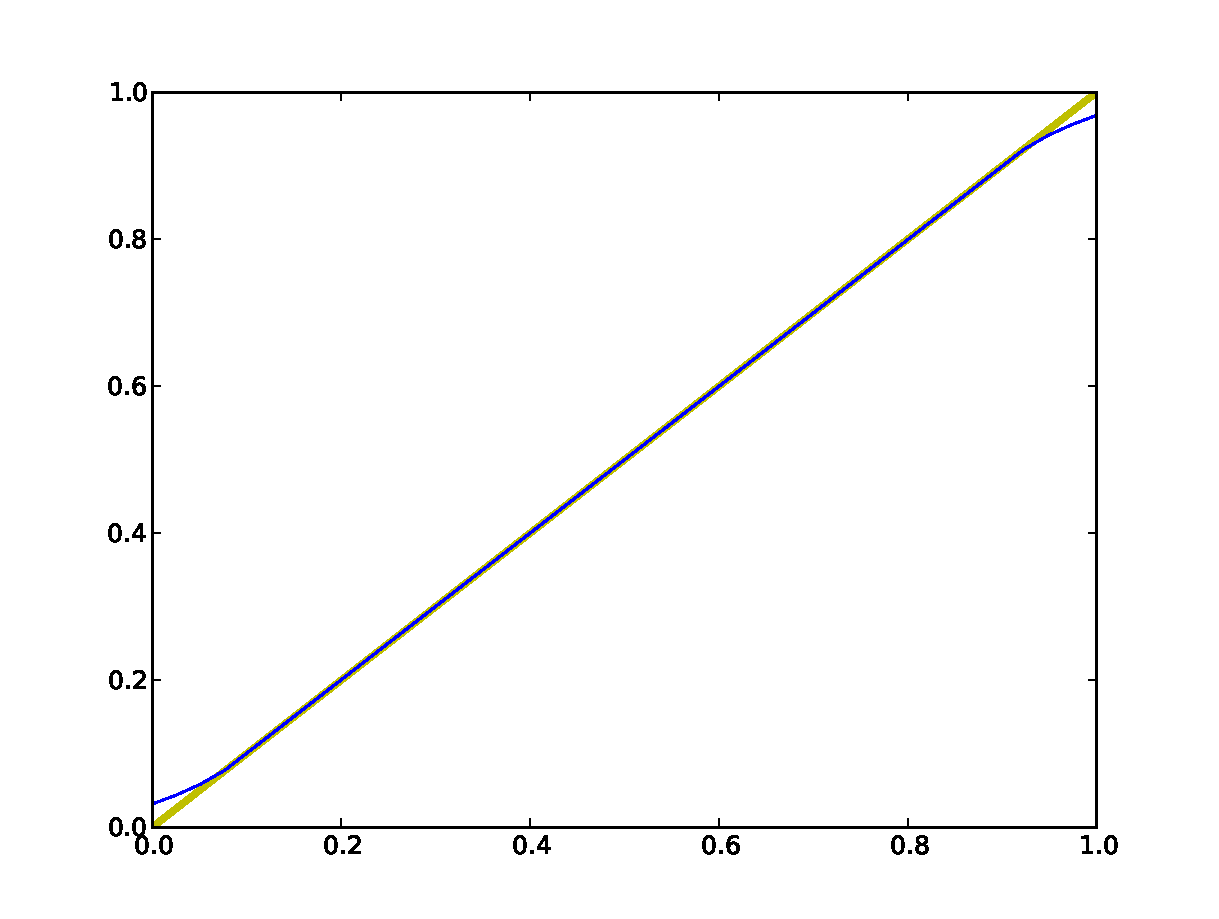
\includegraphics[width=80mm]{figs/linefit.pdf}
  \caption[Fitting a line with a kernel smoother]
  {The result of trying to fit a line with a local-averaging kernel
    smoother.
    Note how the fit is good in the interior but not at the boundaries.
    This is a well known flaw of kernel smoothers.}
  \label{fig:linefit}
\end{figure}

\begin{figure}[!!!ht]
  \centering
    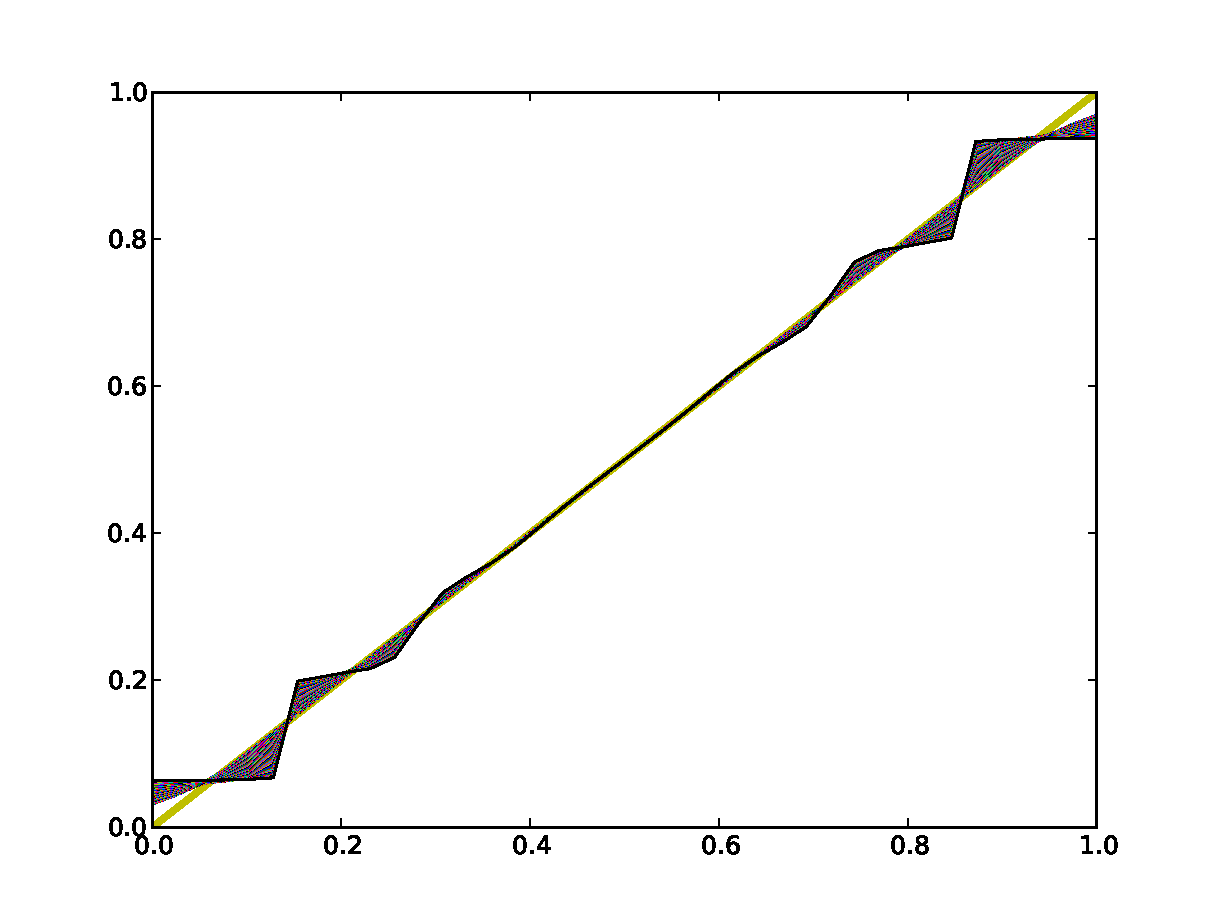
\includegraphics[width=80mm]{figs/linefitmid.pdf}
  \caption[Line fit error getting amplified]
  {In an effort to make $\tilde f$ linear, \textit{DAIWT} squashes
    the ends of the domain, amplifying the error and making the fit
	worse on successive iterations.}
  \label{fig:linefitmid}
\end{figure}

\begin{figure}[!!!ht]
  \centering
    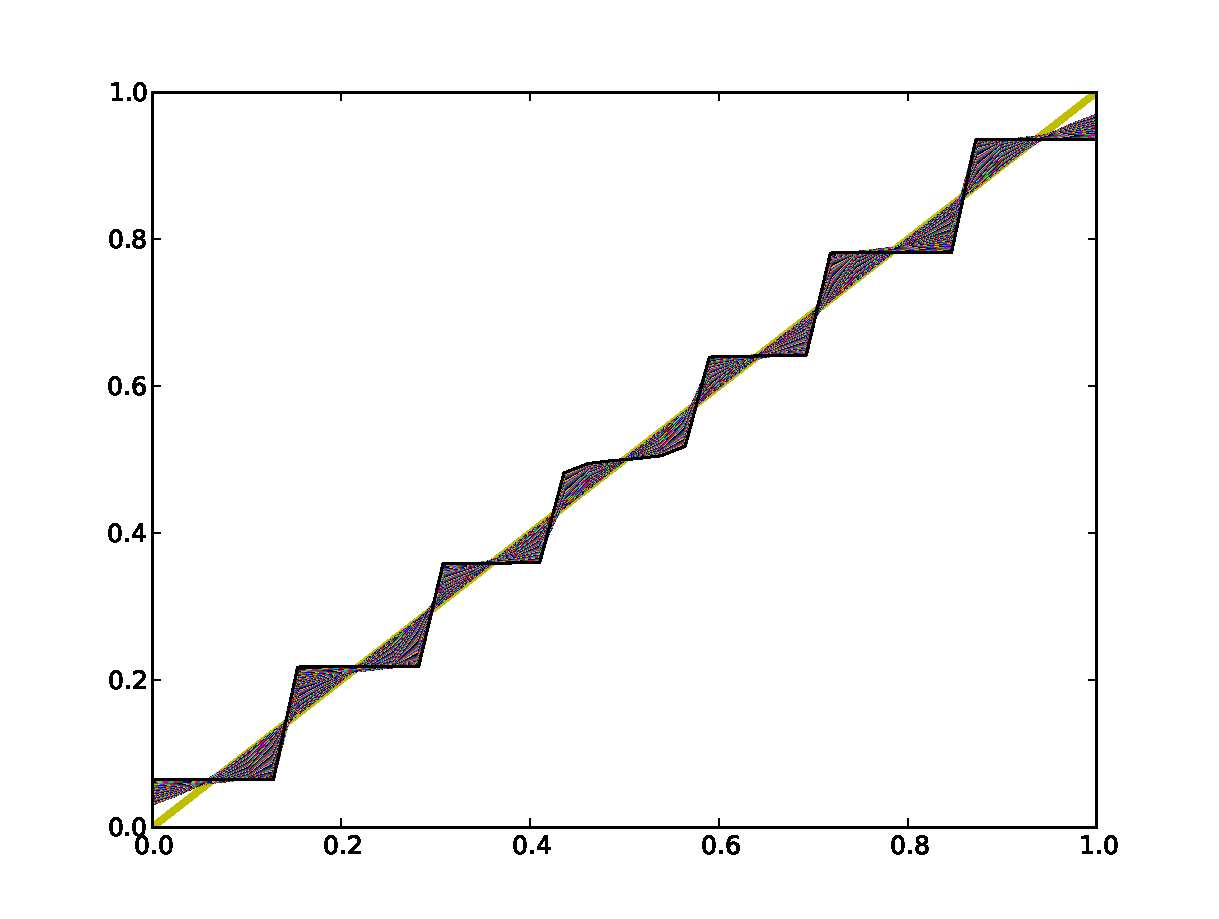
\includegraphics[width=80mm]{figs/linefitend.pdf}
  \caption[Fixed point of FIIRA]
{The process converges to a piecewise flat approximation.}
  \label{fig:linefitend}
\end{figure}

\begin{figure}[!!!ht]
  \centering
    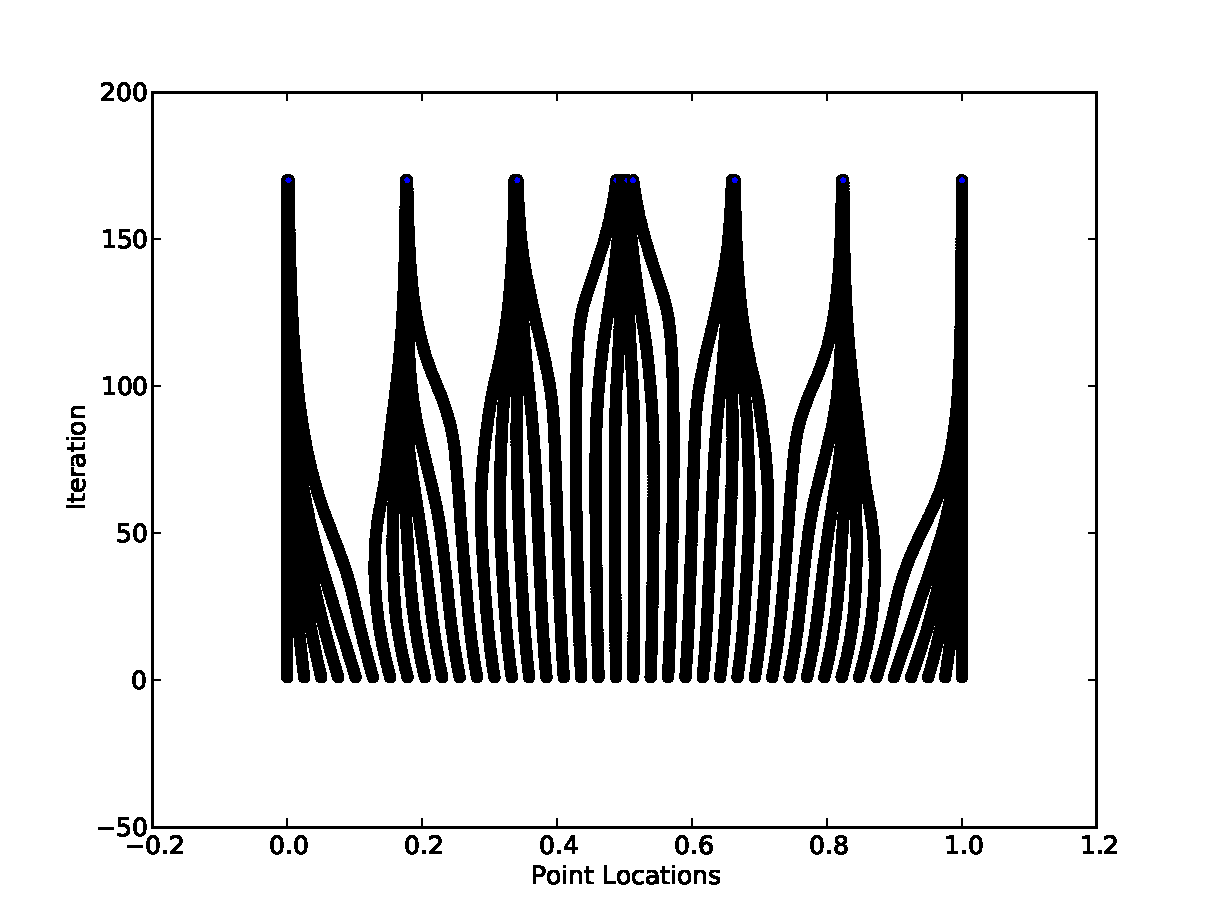
\includegraphics[width=100mm]{figs/linecon.pdf}
  \caption[FIIRA convergence]{How the domain collapses over time.
   First the points near the boundary move closer together,
   then the entire domain collapses to seven atoms.
   Had a smaller bandwidth been used, there would have been more atoms.}
  \label{fig:linecon}
\end{figure}

The reason FDK converges to a piecewise flat approximation is because
kernel smoothers make a local flatness assumption.
The inability of kernel smoothers to represent boundaries and curvature
well is a well-known problem.
A workaround is to use locally weighted regression instead of local
averaging \cite{kercar}.
Locally weighted regression would fix the bias at the boundaries and
just might prevent the piecewise flat convergence.
As noted Ormoneit \& Sen \cite{kbrl} KBRL can be modified to use regression,
but I do not explore that option in this thesis.

The fact that FDK converges to a piecewise flat approximation is not a
damning result.
For many functions, the fit gets better before it gets worse.
We merely stop the process when the best fit is obtained.
Figures 4-6 and beyond show the result when the algorithm is applied to 
a few different functions.

The plots on the left show the function being approximated (yellow), the kernel
smoother fit of the function (blue), the best FDK fit obtained (red), and the fixed
point function to which FDK converges for the value of $\alpha$
that produced the best fit (green).
The plots on the right show how the approximation error changes over
time for different values of $\alpha$.
Approximation error is measured as the sum of squared errors on the points
in the dataset used to generate the fits normalized so that the fit produced
by a the kernel smoother has unit error.

\begin{figure}[!htb]
  \minipage{0.5\textwidth}
    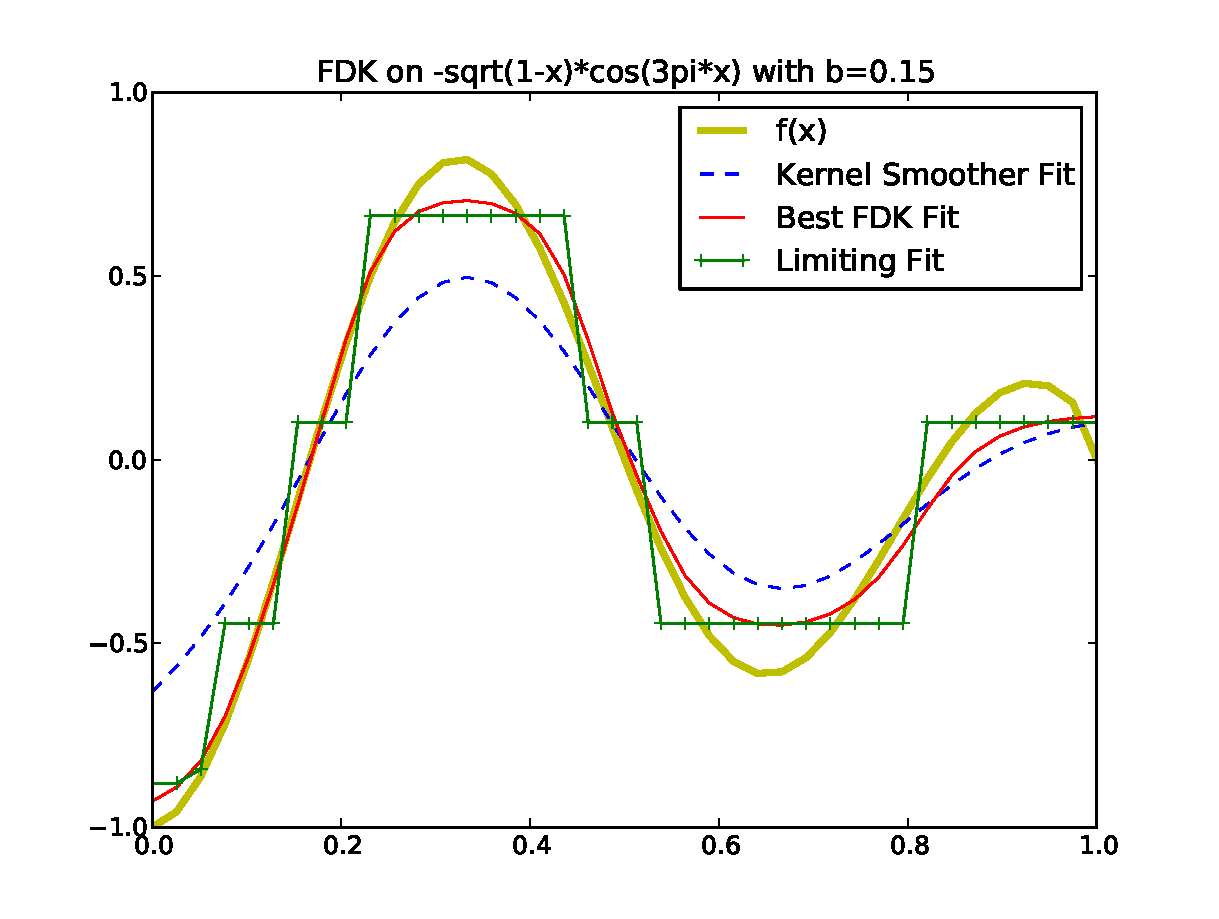
\includegraphics[width=\linewidth]{figs/chap4/sqcos.pdf}
  \endminipage\hfill
  \minipage{0.5\textwidth}
    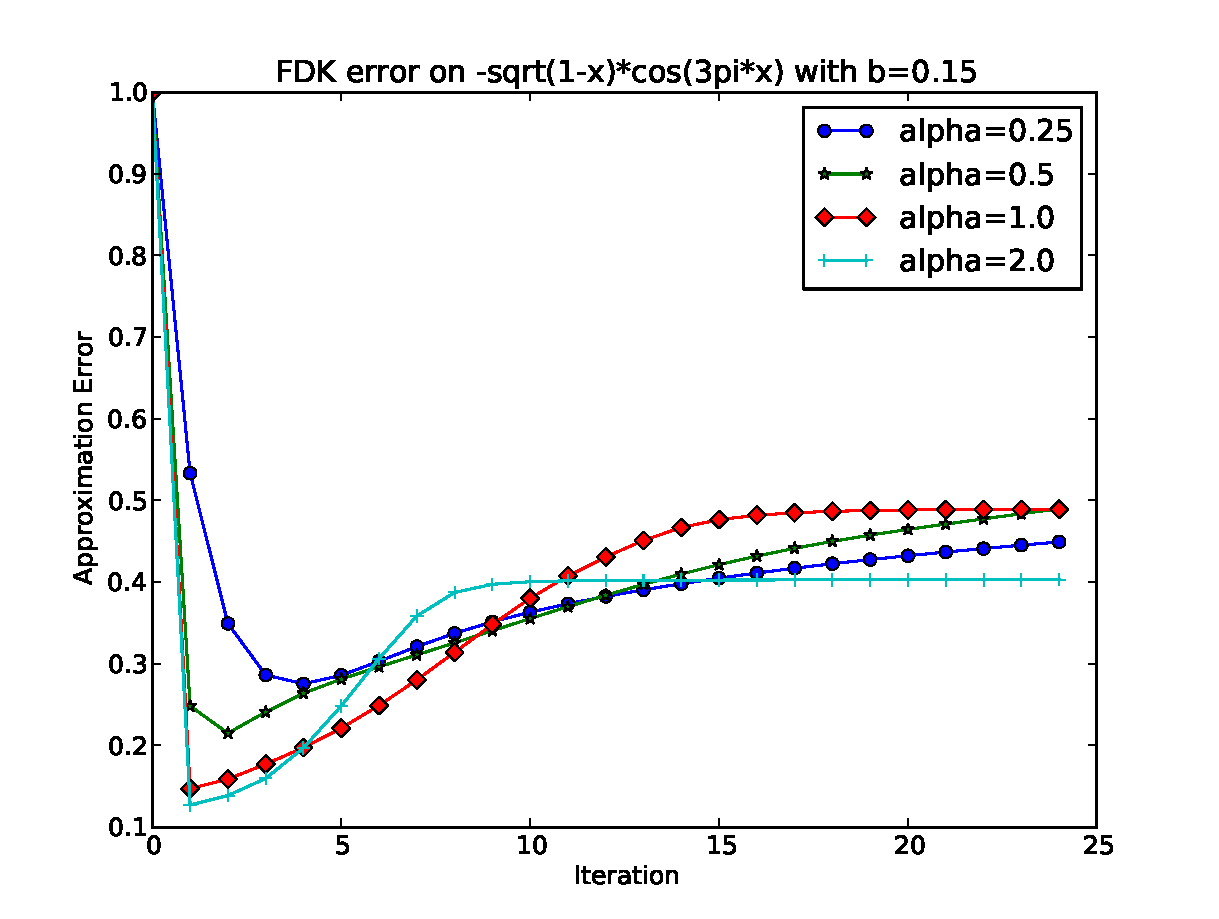
\includegraphics[width=\linewidth]{figs/chap4/sqcoserr.pdf}
  \endminipage
\caption[Fitting $-\sqrt{1-x}\cdot\mathrm{cos}(\pi x)$]
{FDK fit for $-\sqrt{1-x}\cdot\mathrm{cos}(\pi x)$.}
\end{figure}

\begin{figure}[!htb]
  \minipage{0.5\textwidth}
    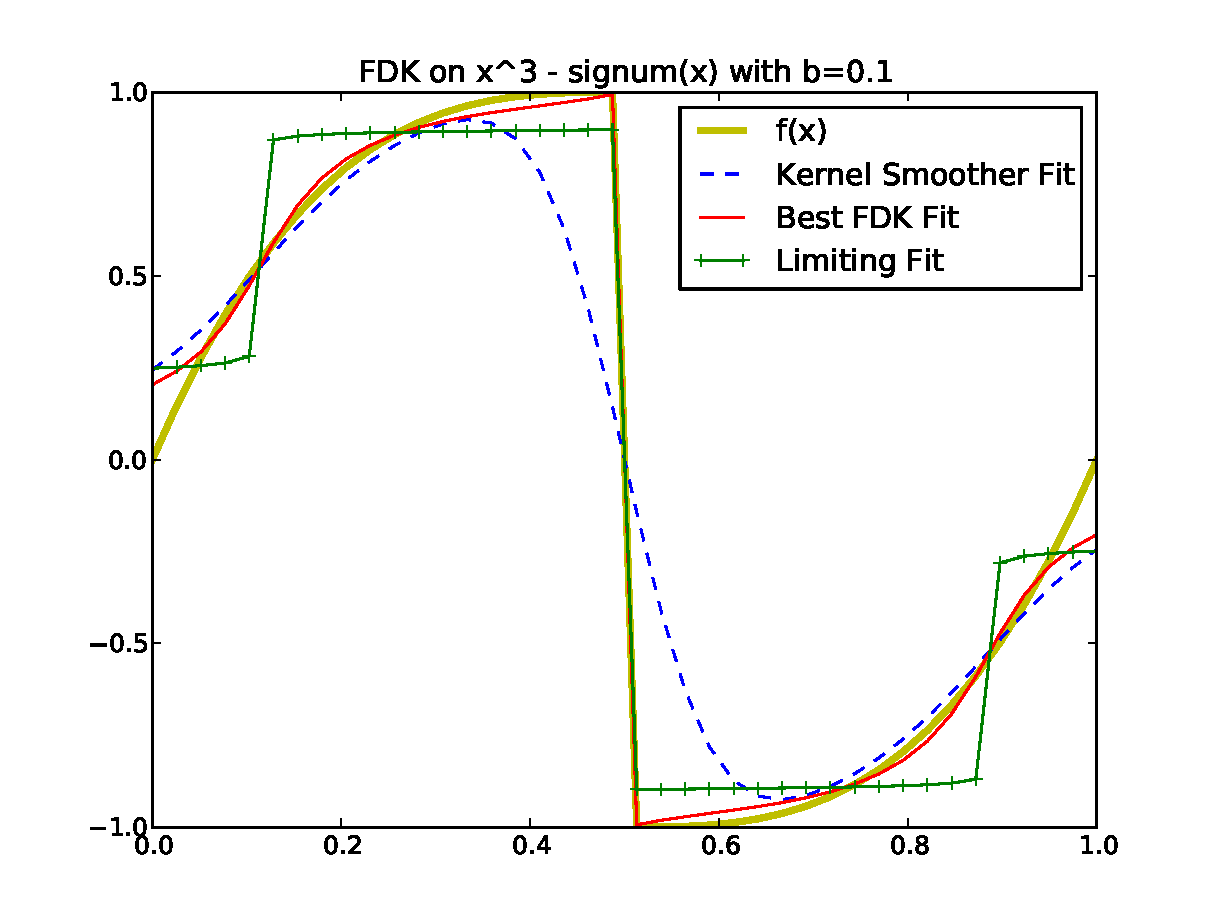
\includegraphics[width=\linewidth]{figs/chap4/flip.pdf}
  \endminipage\hfill
  \minipage{0.5\textwidth}
    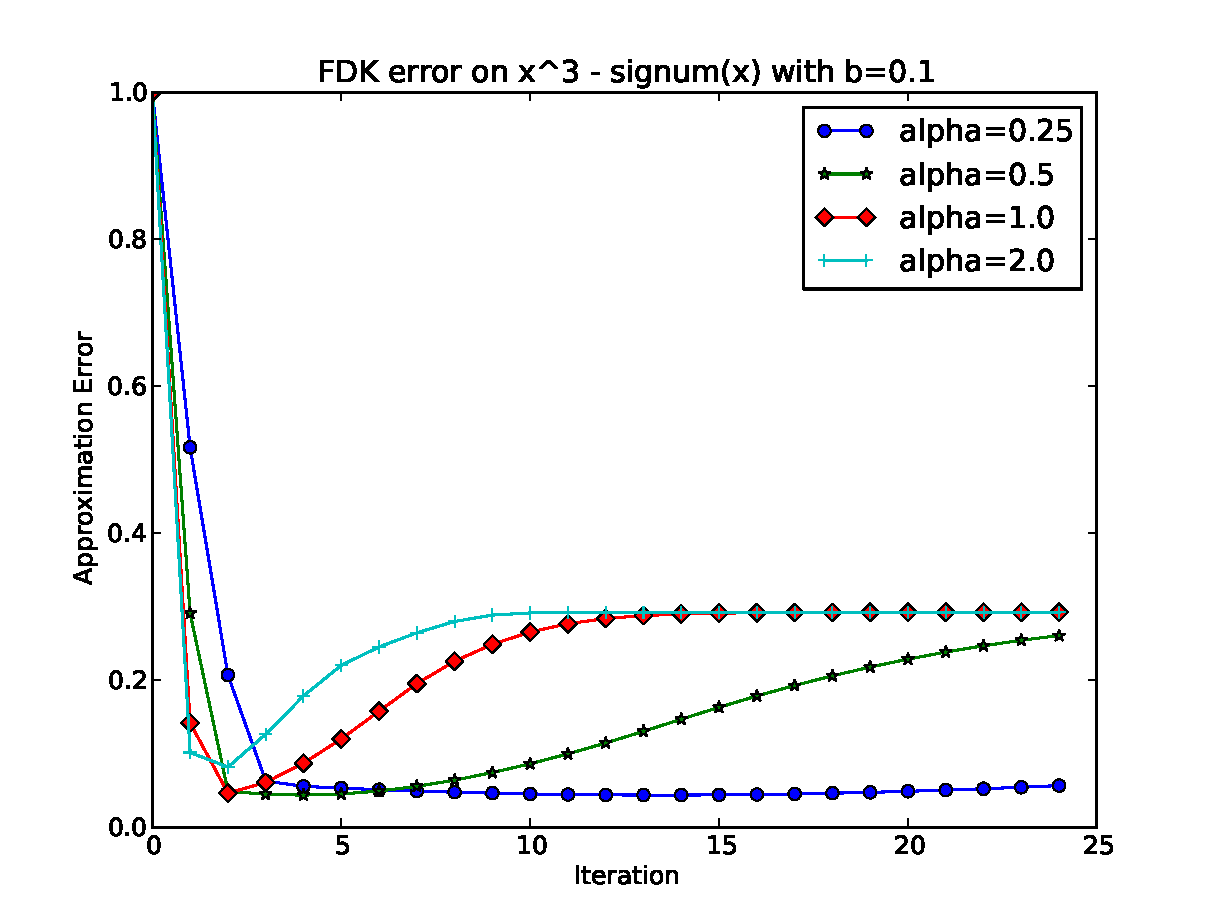
\includegraphics[width=\linewidth]{figs/chap4/fliperr.pdf}
  \endminipage
\caption[Fitting $x^3 - \mathrm{signum}(x)$]
{The same as above but here the function is $x^3 - \mathrm{signum}(x)$}
\end{figure}

\begin{figure}[!htb]
  \minipage{0.5\textwidth}
    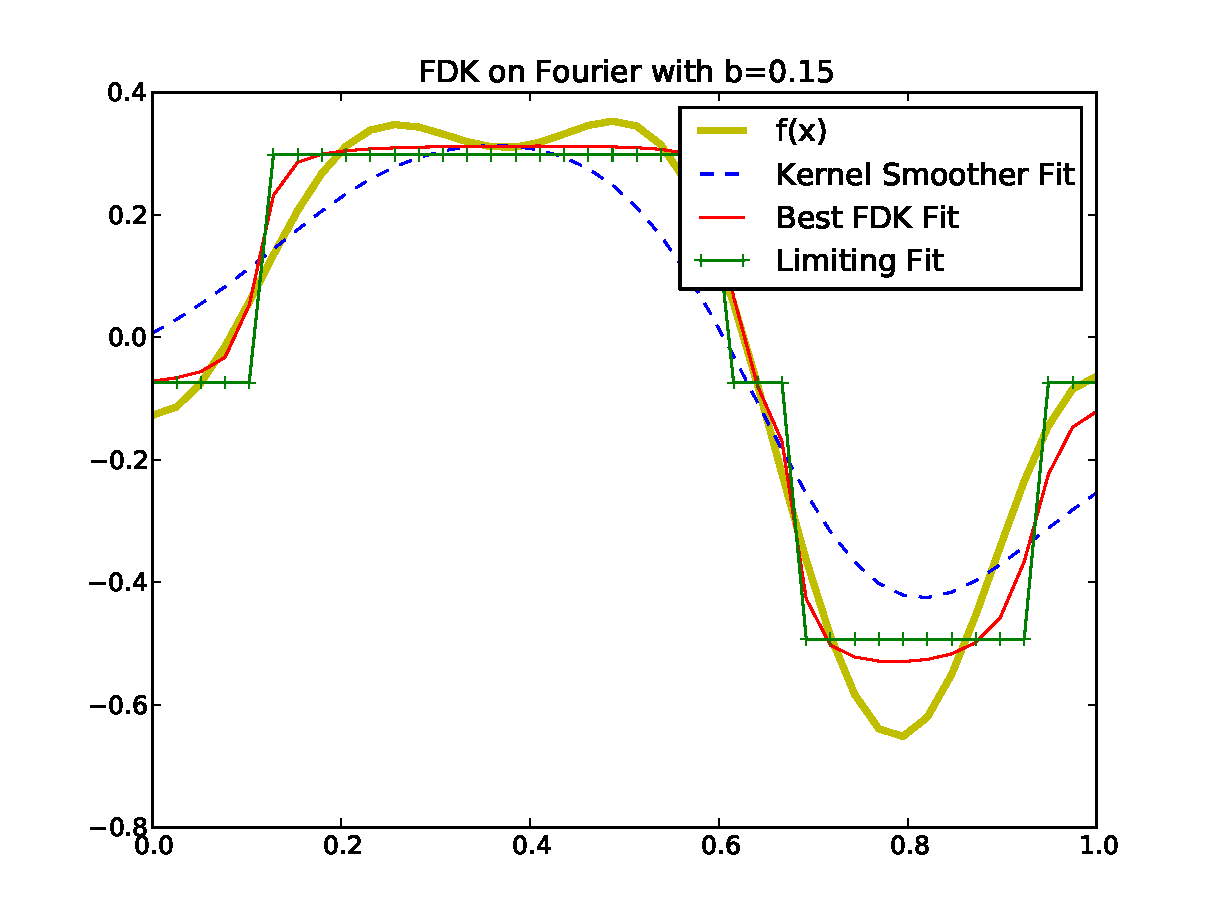
\includegraphics[width=\linewidth]{figs/chap4/bump15.pdf}
  \endminipage\hfill
  \minipage{0.5\textwidth}
    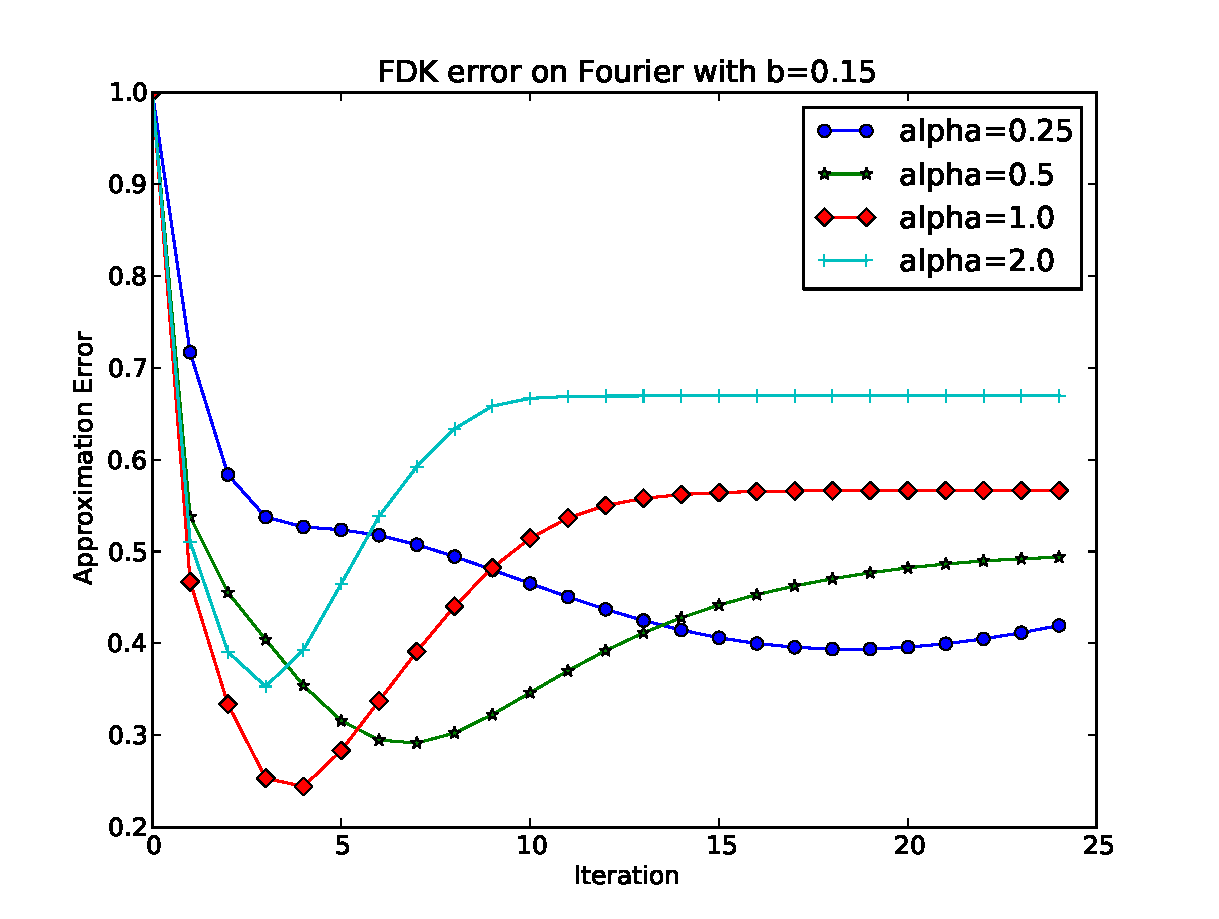
\includegraphics[width=\linewidth]{figs/chap4/bump15err.pdf}
  \endminipage
\caption[Fitting an order 5 Fourier function with $b = .15$]
{The same as above but here the function is some order 5 Fourier.}
\end{figure}


\begin{figure}[!htb]
  \minipage{0.5\textwidth}
    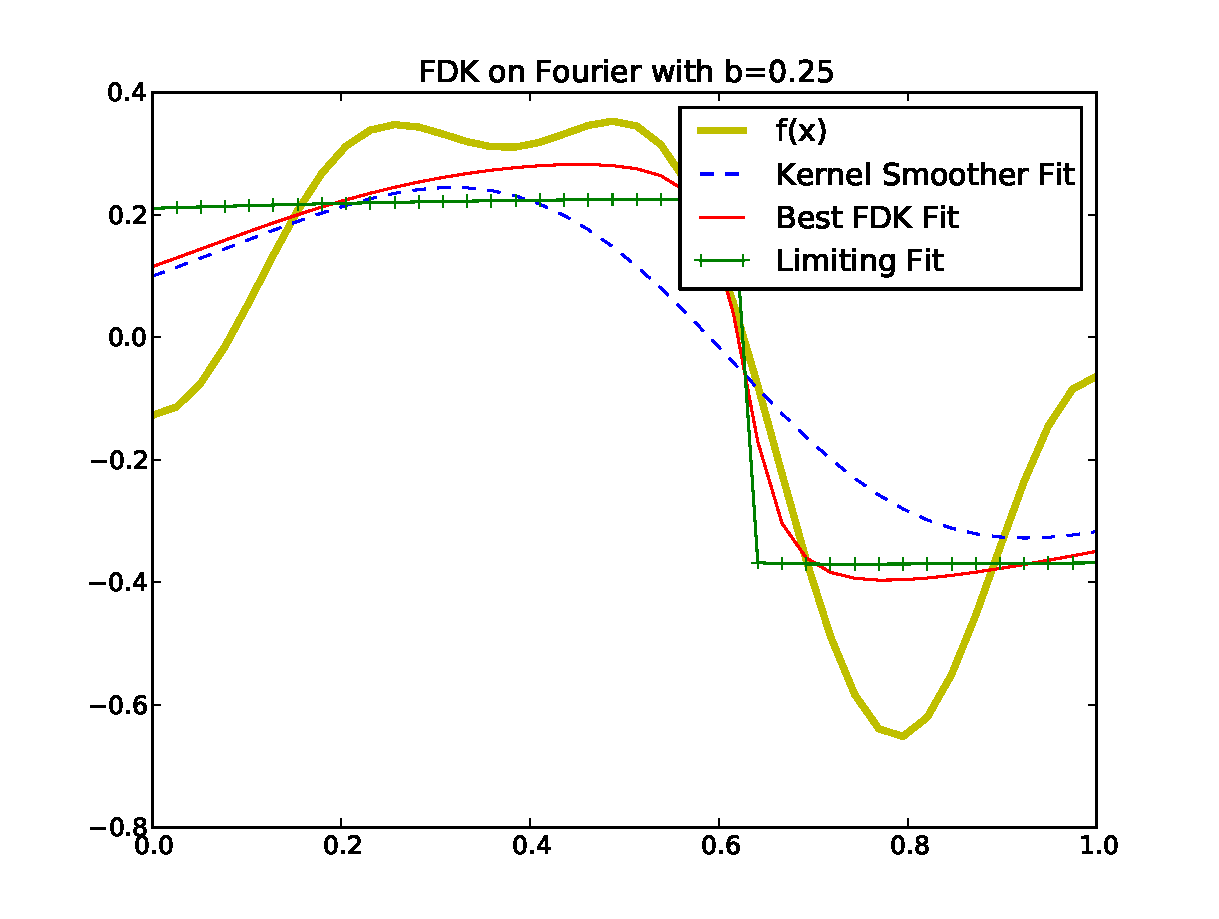
\includegraphics[width=\linewidth]{figs/chap4/bump25.pdf}
  \endminipage\hfill
  \minipage{0.5\textwidth}
    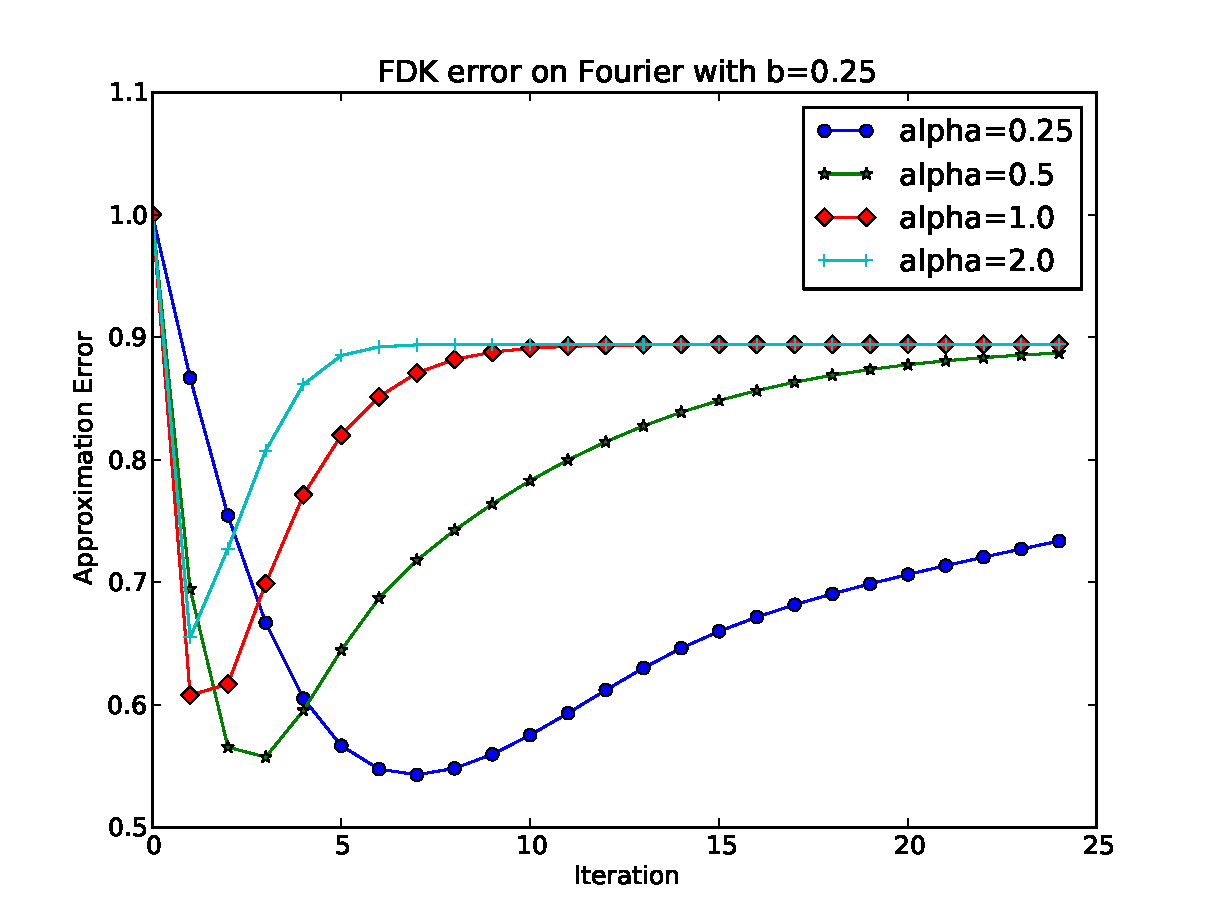
\includegraphics[width=\linewidth]{figs/chap4/bump25err.pdf}
  \endminipage
\caption[Fitting an order 5 Fourier function with $b = .25$]
{The same function as above, this time fit with a different bandwidth.}
\end{figure}

\begin{figure}[!htb]
  \minipage{0.34\textwidth}
    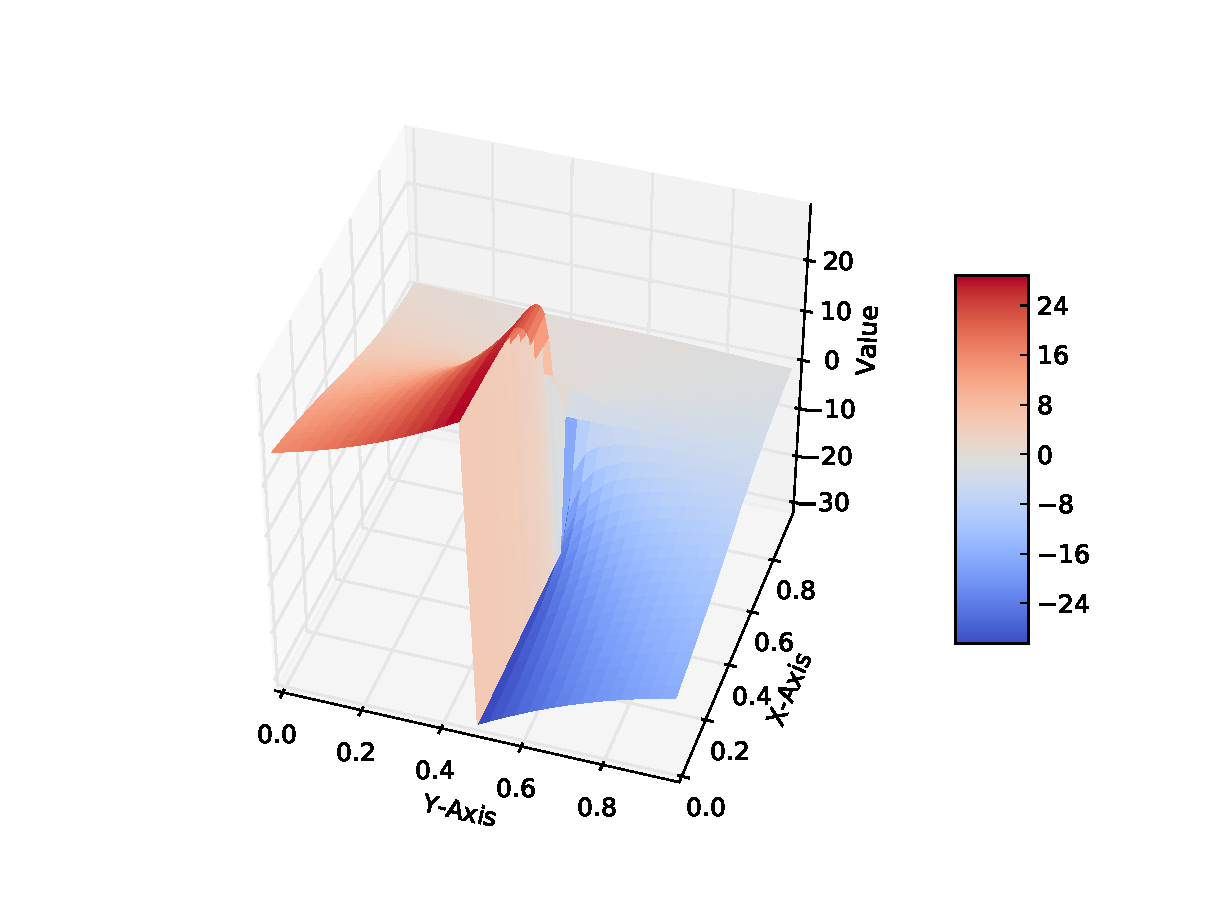
\includegraphics[width=\linewidth]{figs/chap4/atan.pdf}
  \endminipage\hfill
  \minipage{0.33\textwidth}
    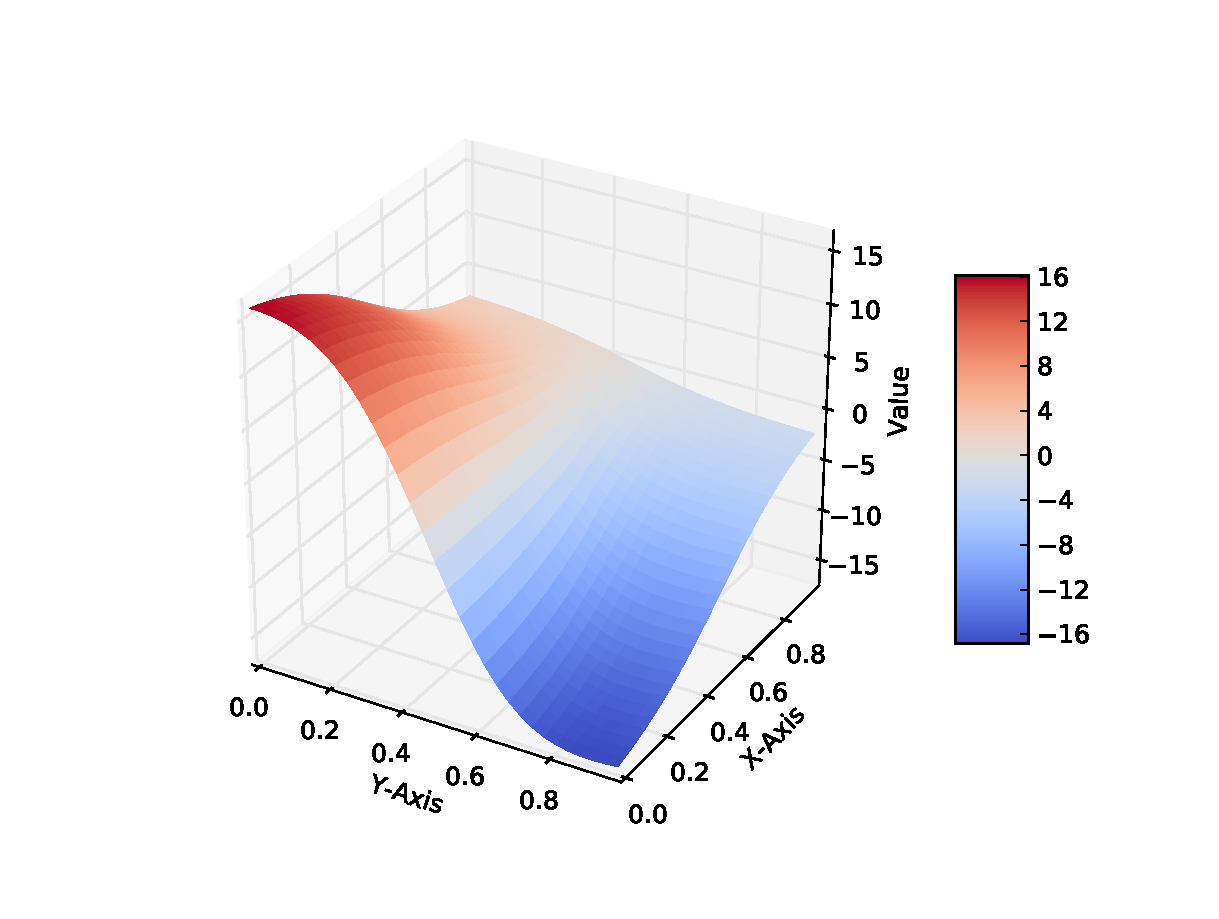
\includegraphics[width=\linewidth]{figs/chap4/atan3s.pdf}
  \endminipage
  \minipage{0.33\textwidth}
    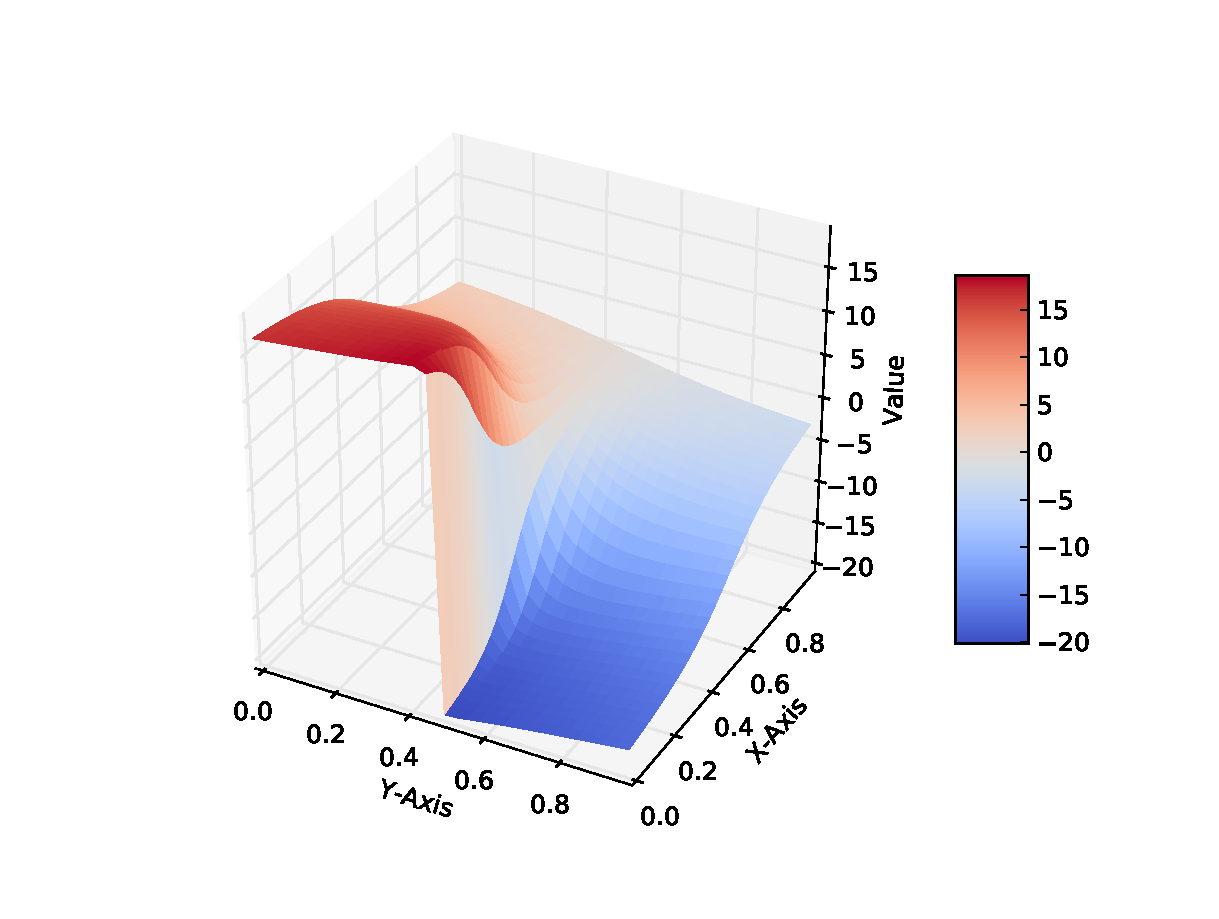
\includegraphics[width=\linewidth]{figs/chap4/atan3e.pdf}
  \endminipage
\caption[Fitting the arctan]{Fitting $f(x,y) = \tan^{-1}(x - .7, y - .5)^3$
Left is the function, mid is the kernel smoother fit, right is the FDK fit.}
\end{figure}

\begin{figure}[!!!ht]
  \centering
    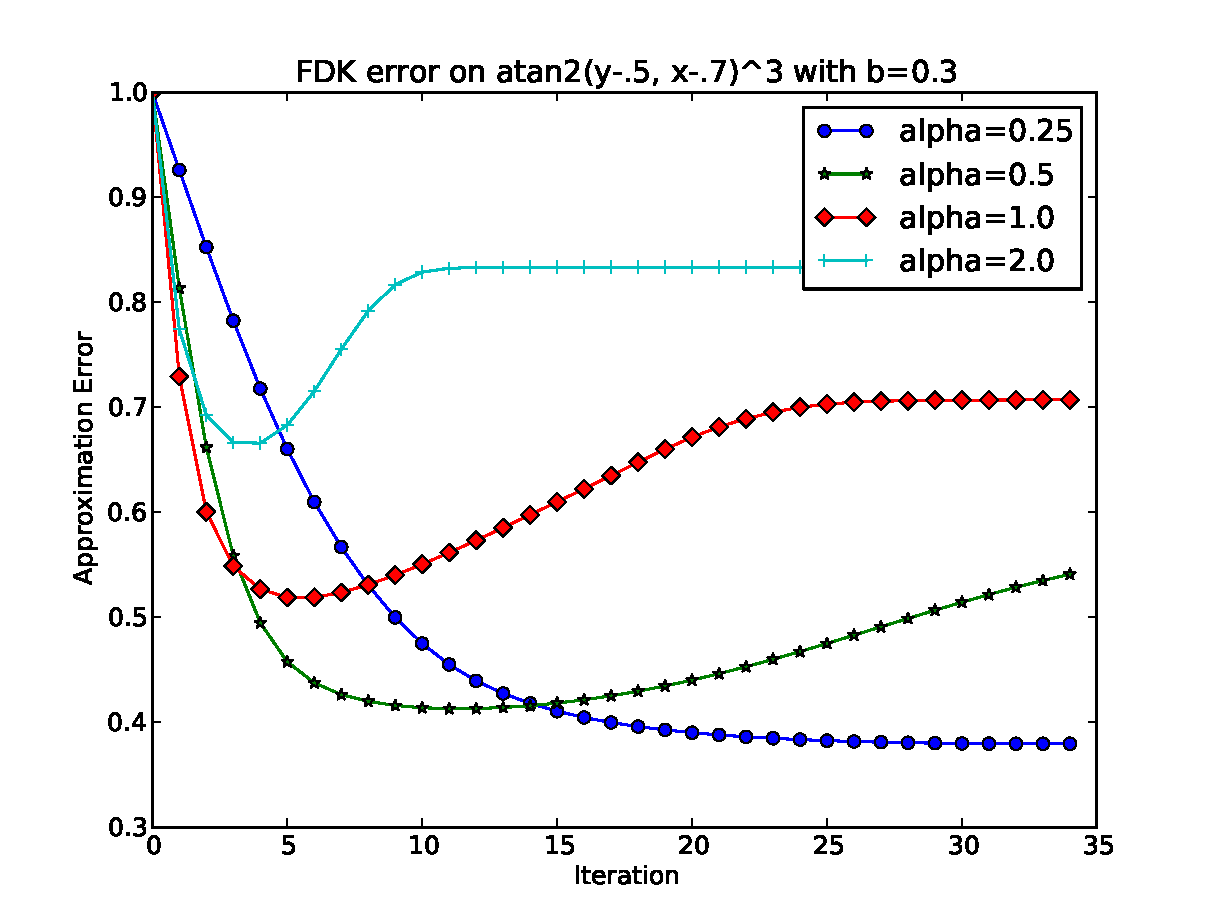
\includegraphics[width=80mm]{figs/chap4/atanerr.pdf}
  \caption{Approximation error when fitting the arctan function}
\end{figure}

These plots reveal several interesting properties of FDK.
First note how well FDK can represent functions with discontinuities.
Further note how few iterations it takes to reach the minimum-error
approximation.
Also note that the optimal value of $\alpha$ depends on the function being
approximated and the bandwidth being used.
Finally note that the error in the limit can depend on $\alpha$, this
means tha for different values of $\alpha$, FDK can collapse the domains to
different numbers of atoms.

\section{FIIRA approach to KBRL}
Algorithm 3 describes an FIIRA approach to KBRL.
Its inputs are the sample transitions, $S' = {S^a | a \in A}$, and
the bandwidth, $b$.

\begin{algorithm}
\caption{DAWIT-KBRL}\label{dkbrl}
\begin{algorithmic}[1]
\Procedure{DKBRL}{$S',\ b$}
	\State $\Phi^a_0 \gets x \mapsto x\ \forall a$
	\State $i \gets 0$
	\Repeat
		\State $Q_{i} \gets KBRL(S', b, \Phi_i)$
                \For{$a \in A$}
                    \State $\Phi^a_{i+1} \gets DAWIT(s \mapsto Q_{i}(s,a))$
                \EndFor
		\State $i \gets i+1$
	\Until{$Q_i \approx Q_{i-1}}$
           \Comment{Or until resulting policy stops improving.}
	\State \textbf{return} $Q_{i}$
\EndProcedure
\end{algorithmic}
\end{algorithm}

Note the following three points about line 5.\\
First, KBRL takes a transform as one of its inputs, this is assuming
KBRL has been modified to do all its local averaging in the transformed
space.\\
Second, The same set of sample transitions $S'$ is used on every
iteration of the algorithm.
One of the requirements for correctness in KBRL is that the data uniformly
cover the reachable state space.
To get the same correctness guarantees,
one would need to resample for coverage in the new space on every iteration.
Sampling for coverage in the new space is equivalent to concentrating samples
in the areas of the original space where the value function is steep.
In \textit{TWO-ROOM} this corresponds to drawing more samples near the
wall.\footnote{
In the analogy from Chapter 1, it corresponds to eating more bell peppers and
jalepe\~{n}os just to pinpoint the difference.}
This is a sensible thing to do because that is how one pinpoints the location
of the wall\\
Third, the regressor used does not have to be KBRL.
It could just as easily be KBSF or iKBSF.

We can see how DKBRL transforms the state space by trying it on
\textit{TWO-ROOM}. The figures show DKBRL discovering and opening up
the wall.

\begin{figure}[!htb]
  \minipage{0.34\textwidth}
    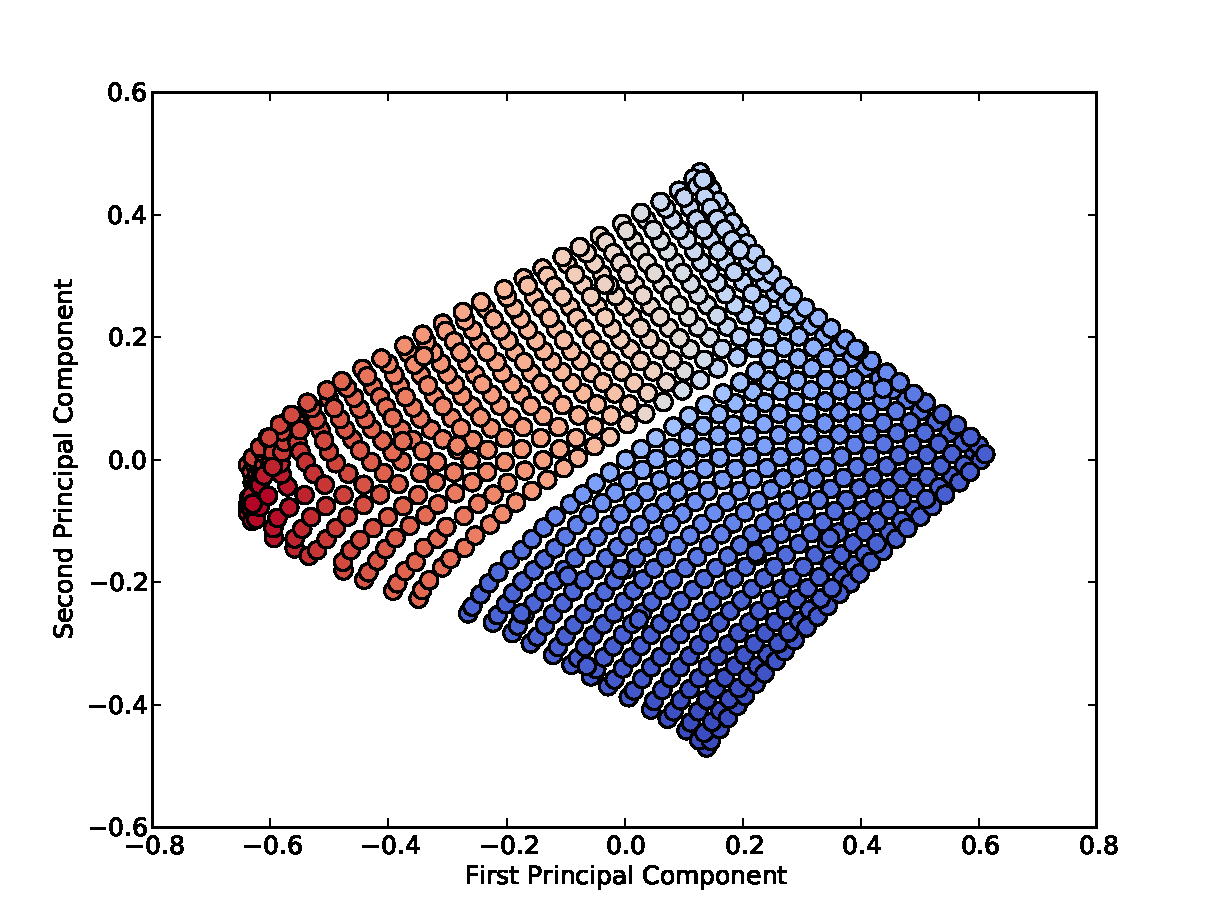
\includegraphics[width=\linewidth]{figs/chap4/2rmop1.pdf}
  \endminipage\hfill
  \minipage{0.33\textwidth}
    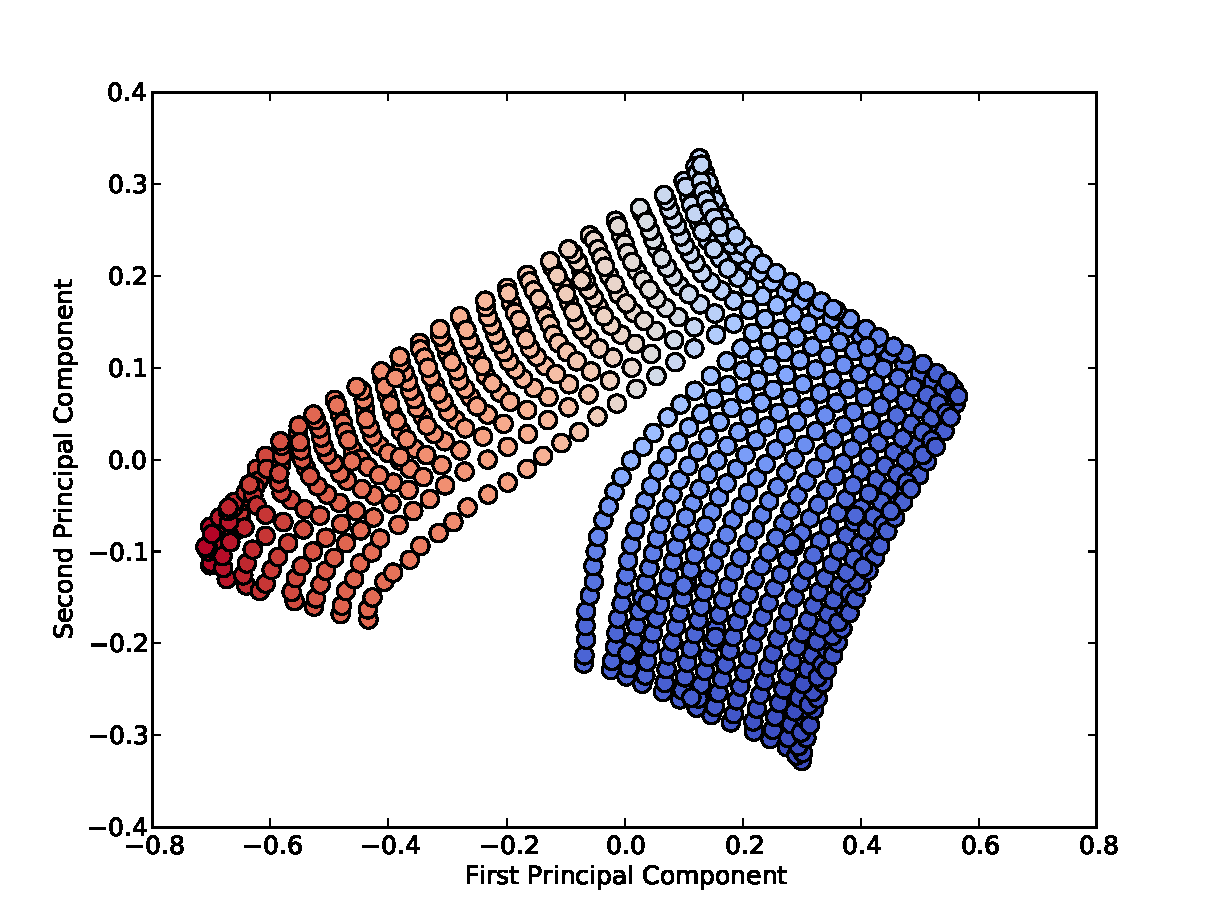
\includegraphics[width=\linewidth]{figs/chap4/2rmop2.pdf}
  \endminipage
  \minipage{0.33\textwidth}
    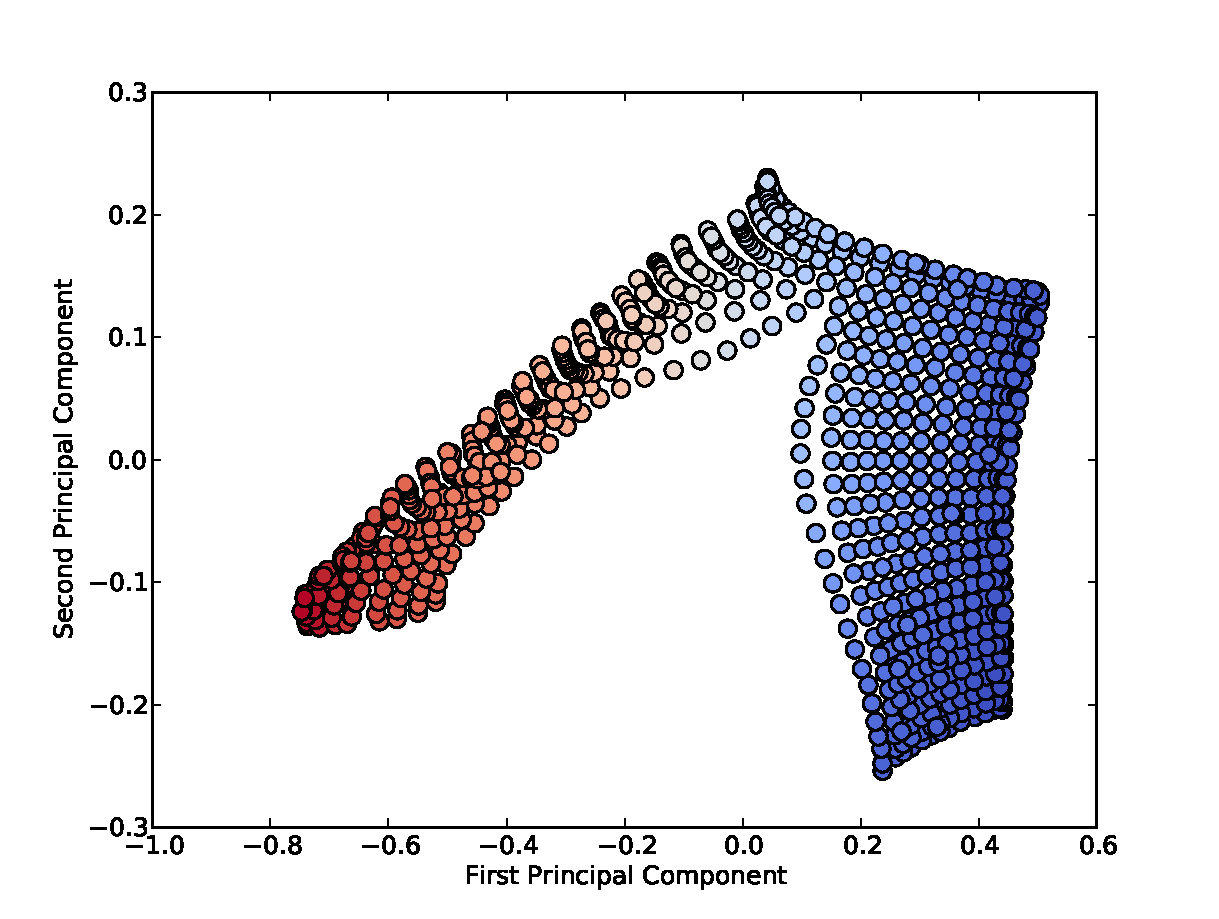
\includegraphics[width=\linewidth]{figs/chap4/2rmop3.pdf}
  \endminipage
\caption[DKBRL opening the wall in \textit{TWO-ROOM}]
{DKBRL opening the wall in \textit{TWO-ROOM} over three iterations.
The first iteration is on the left, it shows the algorithm has started pulling
points apart.
The third iteration is on the right, points are now completely separated by
value.
The points are coloured by their true value.
Note that this is a projection of the transformed space onto two dimensions.
This is why the red points look so squashed.
Along the third principal component (not shown) the red points do not
stack on top of each other as suggested by these pictures.}
\end{figure}

\begin{figure}[!!!ht]
  \centering
    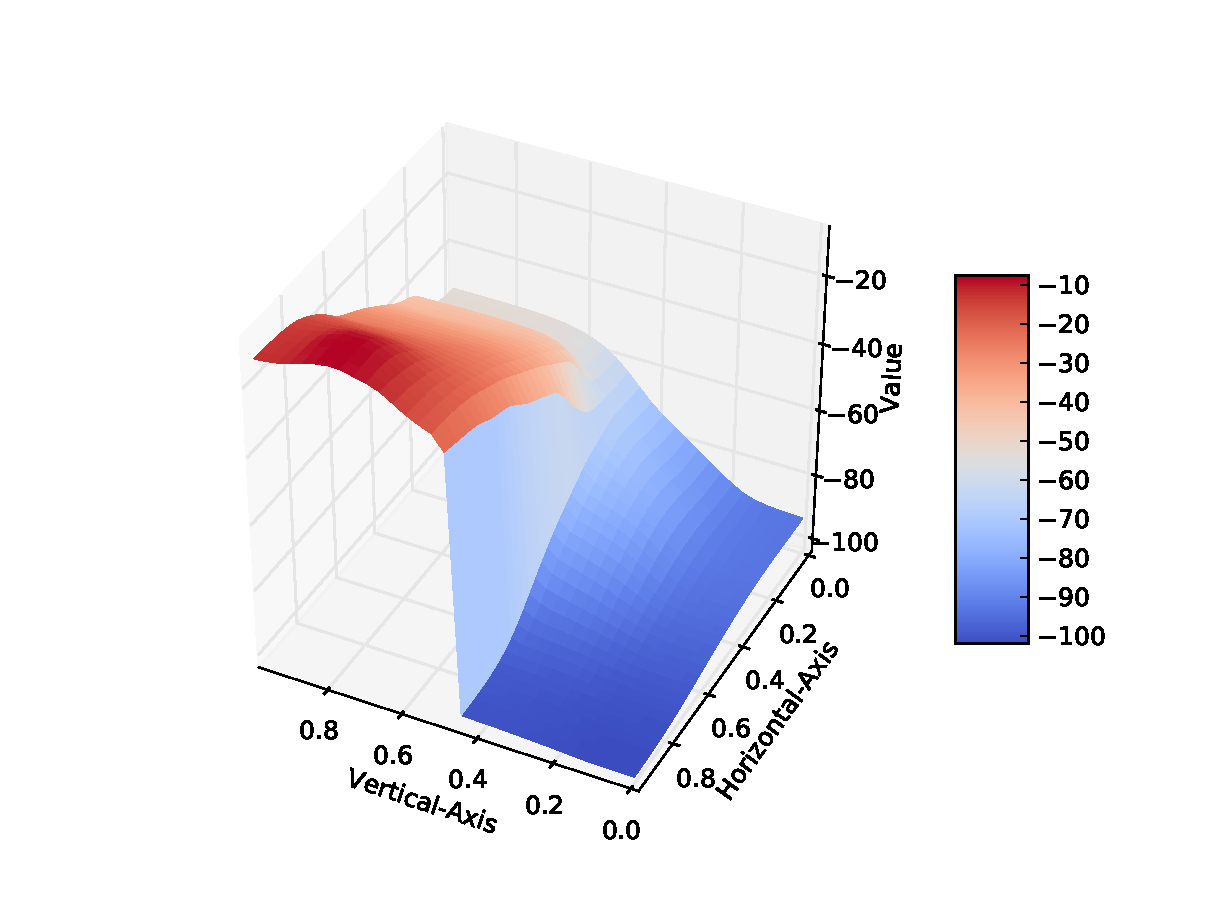
\includegraphics[width=110mm]{figs/chap4/2rmdkb.pdf}
  \caption[DKBRL fit for \textit{TWO-ROOM}]{The fit after three iterations
of KBRL. This was produced with a bandwidth of .06 and the same data as
in Figure 3-3.}
\end{figure}

\section{Implementation Considerations}
In the interest of clarity,
the algorithm descriptions above are not made efficient.
My implementations of these algorithms use the following optimizaions.

When KBRL performs value iteration on the finite model it constructs,
it uses the Q-Values from the previous iteration as a starting point.
This allows for the values to converge faster because the previous
Q-Values are likely to be close to the current ones.

Another optimization is that I do not explicitly compute a transform when
doing FIIRA with a kernel smoother.
Kernel smoothers only need an expression for the distance between points.
So one could do all calculations in terms of
$\mathrm{dist}_i(x_1 - x_2) = \|\Phi_i(x_1) - \Phi_i(x_2)\|$.
This distance can be calculated without $\Phi_i$ using the recursive equation

$$\mathrm{dist}_j(x_1, x_2) = \frac{1}{\sqrt{1 + \alpha^2}}
\sqrt{\mathrm{dist}_{j-1}(x_1, x_2)^2 + \alpha^2\mu_{\tilde f_j}^2
\cdot(\tilde f_j(x_1) - \tilde f_j(x_2))^2}.$$

Note that naively computing distances this way will take time exponential
in $j$, so doing this efficiently requires memoization.

A possible concern about adding dimensions is that it might make the
problem harder. Note that when the dimensions are added, the state space
retains its original dimensionality---it just becomes a manifold
in higher dimensional space.
The performance of kernel regression depends on the dimension of the manifold
and not the dimension of the embedding space.

As a final implementation consideration, note that the space created by the
transform can be visualized using MDS to rotate
the space so the principal components are axis aligned.

My implementations use all of these optimizations. The next chapter shows
the result of applying Algorithm 3 to some benchmark RL problems.
